% !TEX encoding = UTF-8 Unicode 
% !TEX root = praca.tex

\section{Cross-platform mobile development}

As the term suggests, cross-platform or multi-platform frameworks enable to create applications that can be installed on different platforms, and consequently reach a larger user base. There are many solutions available in the market, which all offer support for a narrow or wide subset of existing platforms. Therefore, applications may be published as, e.g., mobile apps (Android, iOS), web apps, desktop apps (Windows, macOS, Linux) or even embedded apps. The number of operating systems tends to increase under the principle of ``write once, run everywhere'' followed by frameworks' creators \cite{comparison_technologies_multiplatform}. 

The main advantage of cross-platform development over native development is in line with its primary goal, which is the ability to create and maintain a single codebase, no matter the number of target platforms. Moreover, as described in the chapter \ref{chap:native}, Android operating system suffers from high level of fragmentation which can be addressed with cross-platform framework as well. Being able to operate on a single codebase results in the development costs decrease. Implementation is more time-efficient without the need to build multiple projects. This remains true for post-release support in the form of updating versions and handling bugs or change requests. Cross-platform approach is also lighter on resources, requiring just a single development team, which additionally removes possible collaboration issues between teams that can occur in native approach. In the past, it would be assumed it is easier to gather an experienced team for native development, however currently the most popular multi-platform frameworks are mature enough to have created active communities with high level of know-how \cite{approach_to_assess_performance_case_study,comparison_perf_looks_flutter_native,comp_analysis_hybrid_frameworks}.

There are differences between available cross-platform frameworks, especially in the context of 
architecture or rendering and compilation method. They will be described in the following chapters. Essentially, most of them require a middle layer that connects the app with the system and translates the commands to be natively called. This is considered to be a possible root of performance decrease \cite{appdynamics_mobile_app_performance}. And although a single workspace is used during development and testing, in order to publish the final application to different app stores (e.g. Google Play Store, App Store), there must be performed a build for each target platform to acquire separate app bundles that can then be uploaded \cite{comp_study_hybrid}.

As explained in the previous chapter, different operating systems usually have different guidelines provided when it comes to user interface (UI) design. This might become an issue depending on design assumptions. Considering the user's point of view, there are three approaches to UI implementation. Firstly, the app appearance may be identical regardless of the platform it runs on. In this case, the platform-specific conventions may not be fulfilled and only when implemented correctly it will not cause user experience decrease. Secondly, the app may have a completely system-compliant look and feel. In this case, the issue may be raised as to how efficient it is to implement disjointed layouts in the cross-platform solution compared to switching to the native approach. Finally, there is an intermediate approach which assumes that most of the app elements are shared between platforms, but there are some that are platform-specific, e.g., popups, action buttons \cite{cross_platform_ux,baseline_cross_platform}.

\begin{figure}[h]
	\centering
	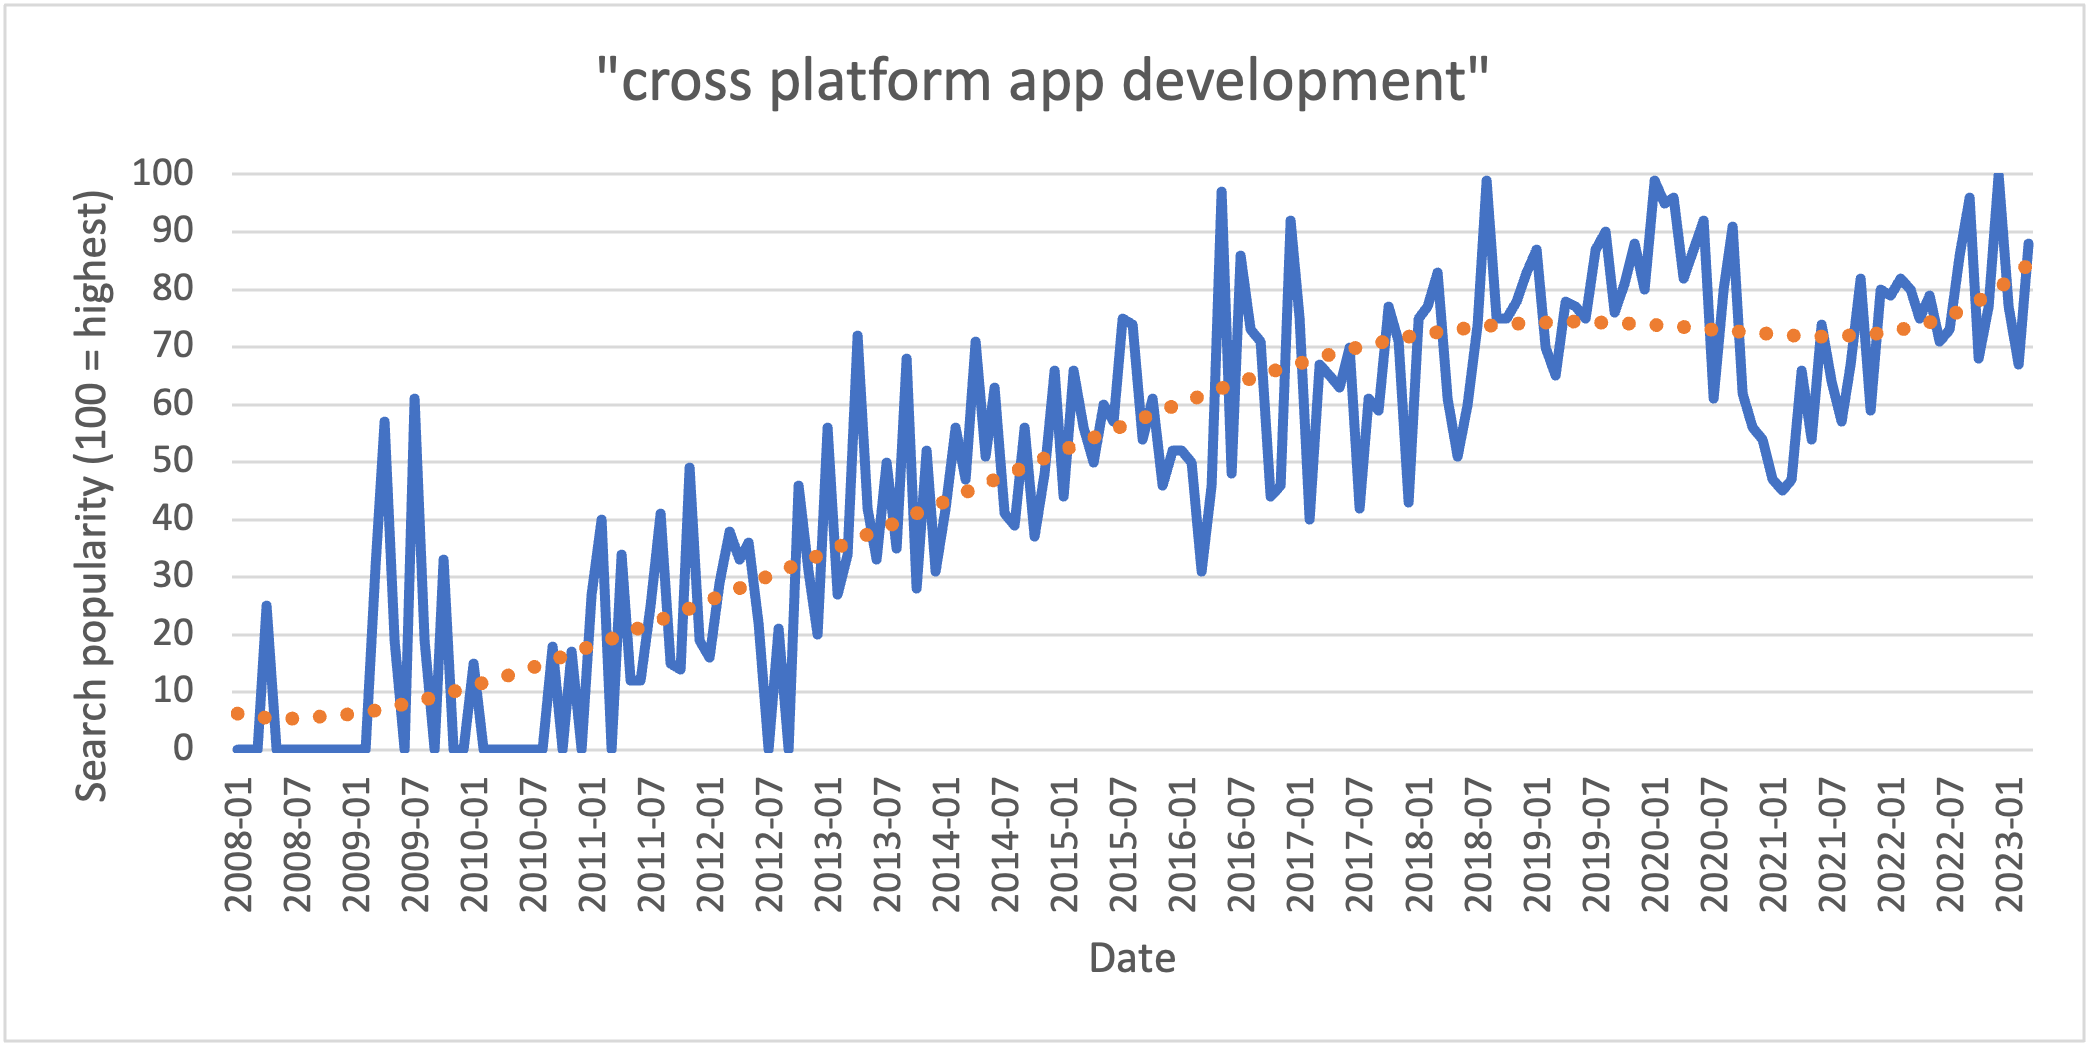
\includegraphics[width=\textwidth]{img/google_trends_cross_platform}
	\caption{Google Trends search popularity of cross-platform app development (Source: Own work based on \cite{trends_cross_platform})}
	\label{fig:trends_cross_platform}
\end{figure}

Despite the existing assumption that cross-platform frameworks might produce applications suffering from performance decrease, their popularity significantly grew during the past couple of years. The Figure \ref{fig:trends_cross_platform} shows the Google search popularity for the phrase "cross platform app development". The upward trend is clearly visible which depicts the big interest in the topic amongst online users. Apache Cordova and Xamarin are examples of multi-platform frameworks which were the most popular in the beginning, however more recent solutions have already surpassed them. In Figure \ref{fig:trends_comparison} the rapid rise of Flutter and React Native can be observed as well as the ongoing importance of Ionic. These three frameworks are different from each other but still share the fact that they gather big user groups. For that reason they have been selected to undergo a review and performance analysis inline with the goal of this thesis.

\begin{figure}[h]
	\centering
	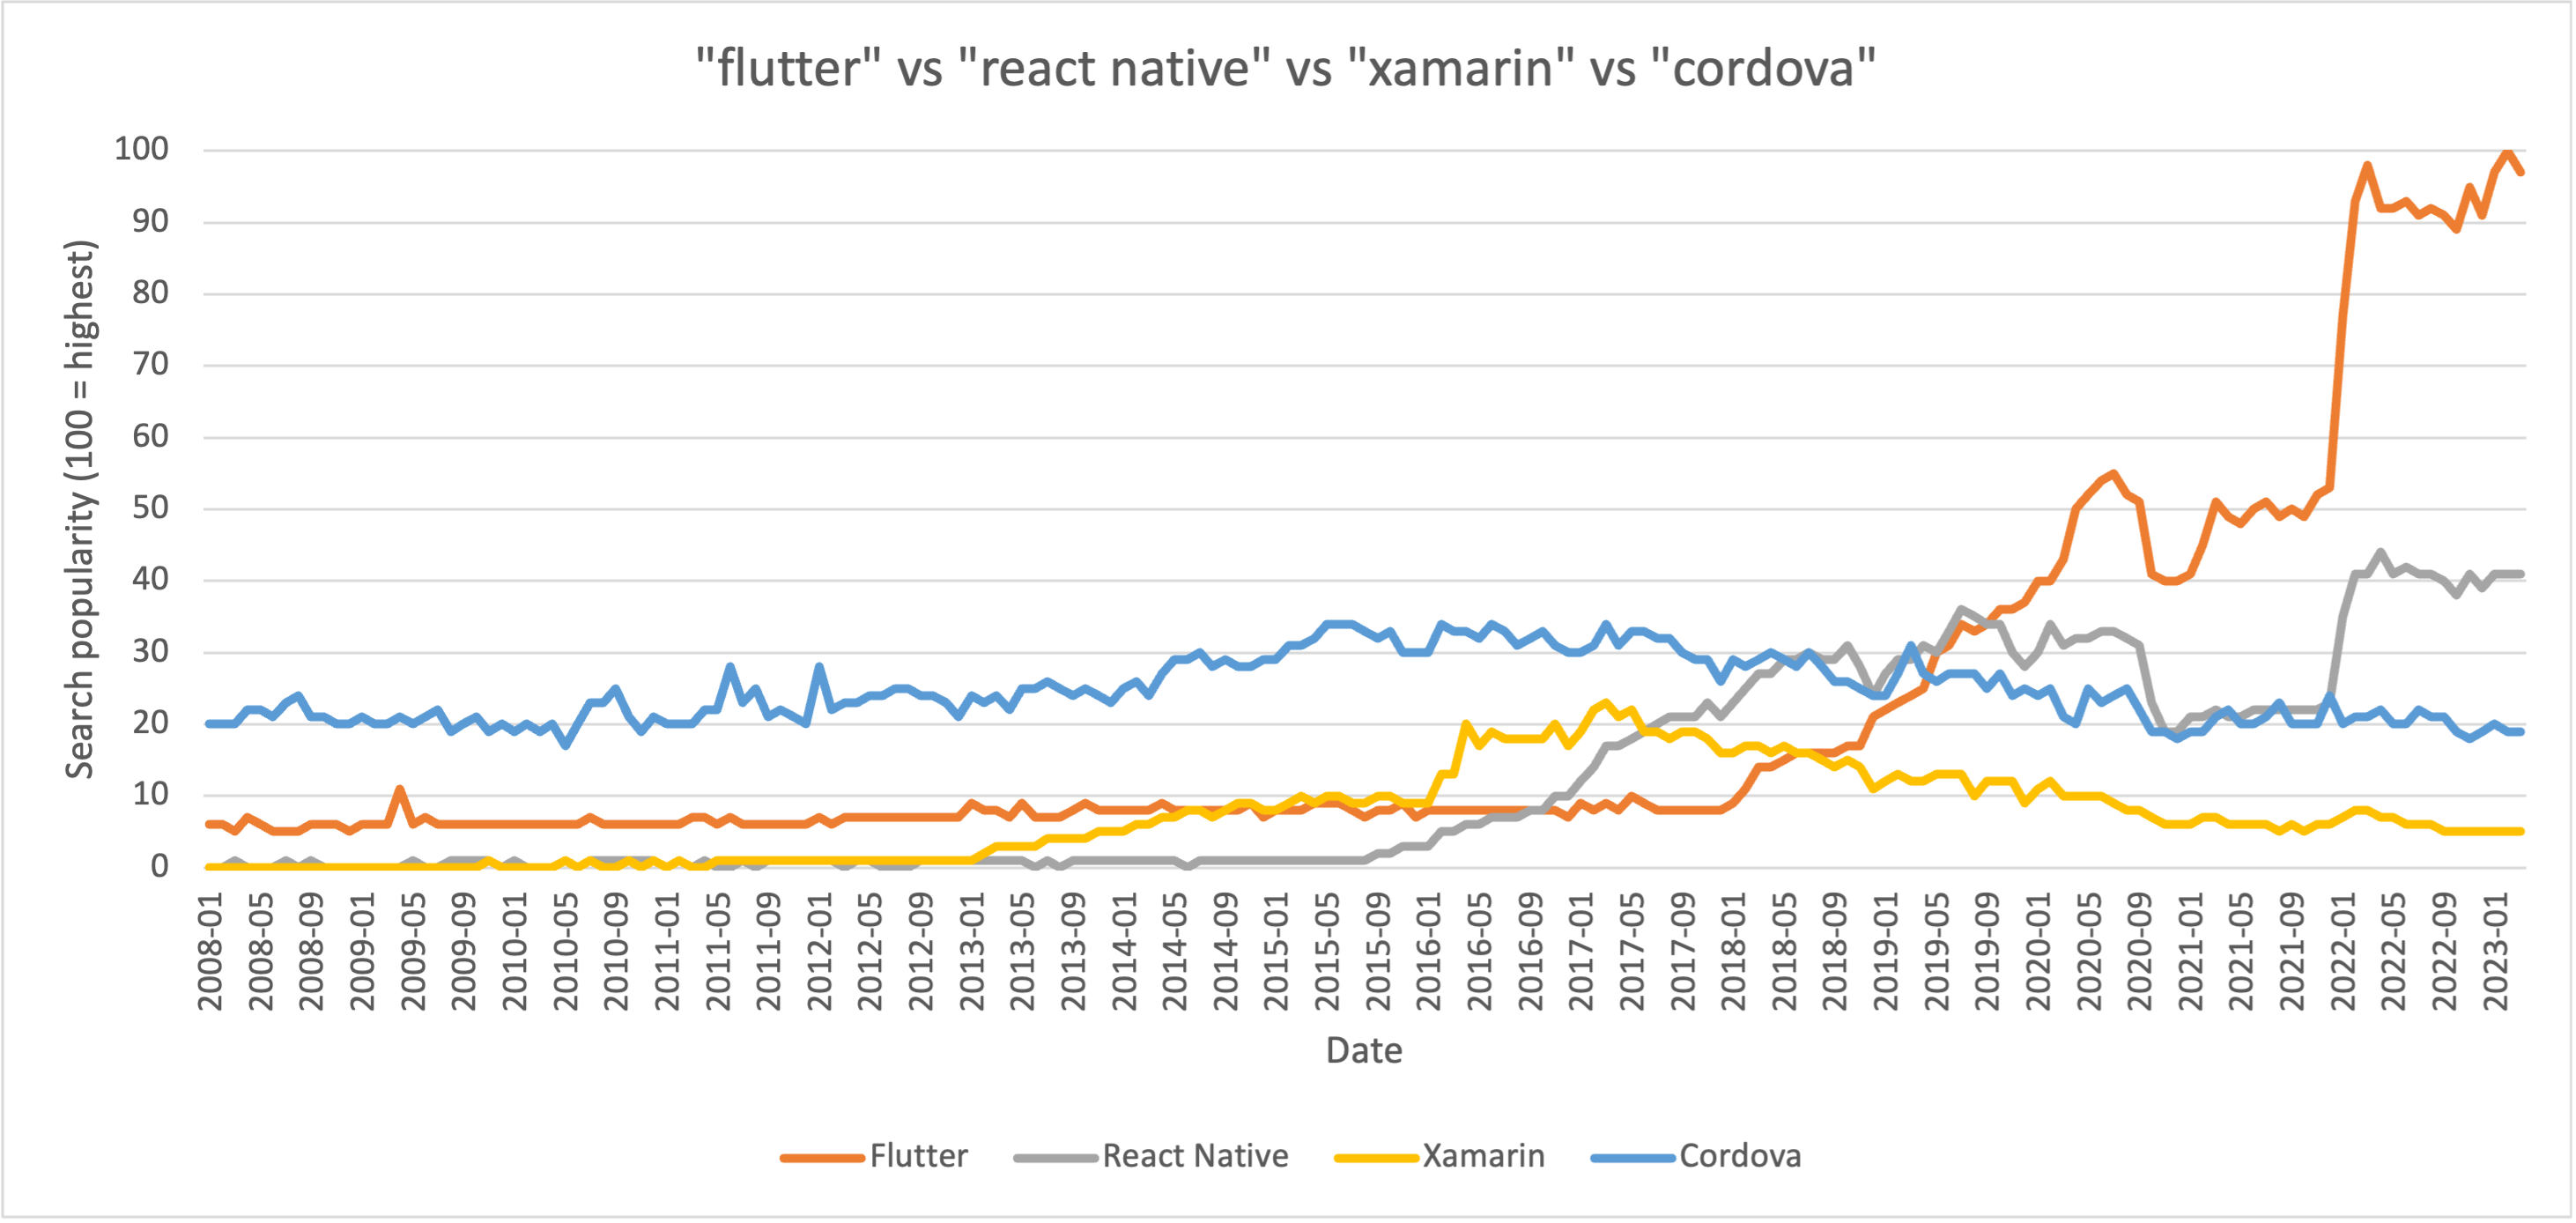
\includegraphics[width=\textwidth]{img/google_trends_comparison}
	\caption{Google Trends search popularity of selected cross-platform frameworks (Source: Own work based on \cite{trends_comparison})}
	\label{fig:trends_comparison}
\end{figure}

Multiple types of cross-platform solutions can be distinguished. The most commonly present in the scientific literature are the following: hybrid, interpreted, cross-compiled, and Progressive Web Apps (PWAs). Native mobile development may provide better connection with native components and services compared to some of the types mentioned above. This may become the cause of lower performance. 

\subsubsection*{Hybrid approach}

The term \emph{cross-platform} tends to be used interchangeably with \emph{hybrid} which technically is incorrect as these are not necessarily synonyms. The hybrid approach to cross-platform development assumes a merge of native and web applications. Typically, the web app is created with the use of web solutions, e.g. HyperText Markup Language (HTML), Cascading Style Sheets (CSS) and JavaScript (JS) which then runs inside a web view component provided by the native app, allowing to publish the end-product in regular app stores. Usually, there is a bridge enabling the usage of device native features which are out-of-scope for JS API. Figure \ref{fig:hybrid_architecture} shows the overall architecture of a hybrid application. One of the drawbacks is that the access to native components is not possible while building the user interface, which makes it more difficult to mimic the native look and feel for the user. The hybrid approach may provide a lower performance for the bigger projects because the application is executed by the browser engine and the bridge may cause overhead \cite{survey_taxonomy_cross_platform,comparison_technologies_multiplatform,cross_platform_development_study_rn_flutter,eval_rn_flutter,comp_analysis_hybrid_frameworks}.

\begin{figure}[h]
    \centering
    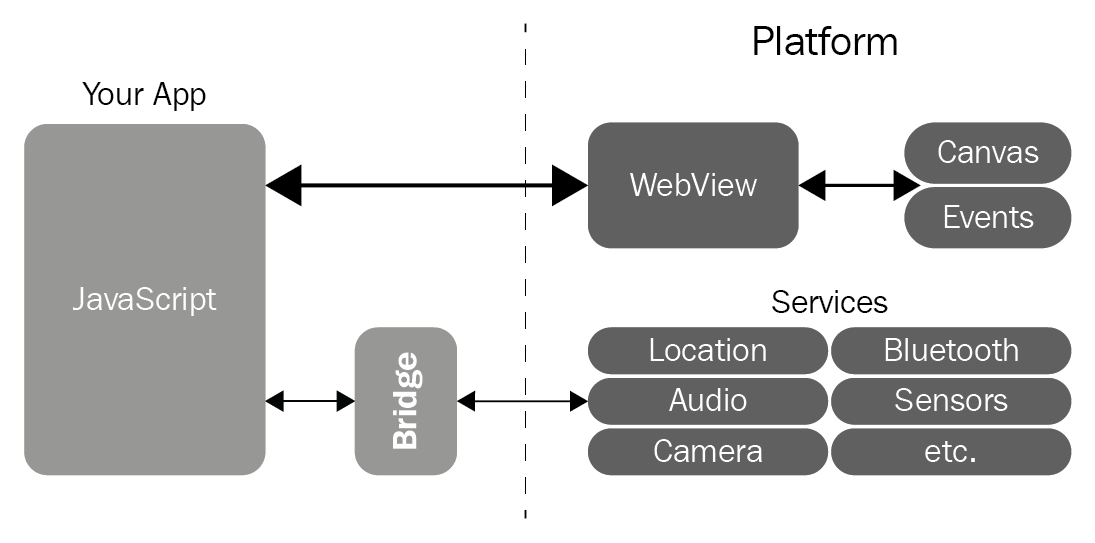
\includegraphics[width=.6\textwidth]{img/hybrid}
    \caption{Hybrid app architecture (Source: \cite{karim_flutter_different})}
    \label{fig:hybrid_architecture}
\end{figure}

\subsubsection*{Interpreted approach}

Similarly to the hybrid approach, web technologies are the primary component of the interpreted approach. The key difference between them is that interpreted apps do not use the web view. Instead, there is an interpreter involved which translates the web elements into native components that can be rendered directly in the operating system. Figure \ref{fig:interpreted_architecture} shows the overall architecture of an interpreted application. In the context of accessing the native features, there is again a bridge applied. The main advantage over the hybrid approach is the guaranteed native appearance and behavior \cite{survey_taxonomy_cross_platform,eval_rn_flutter}.

\begin{figure}[h]
    \centering
    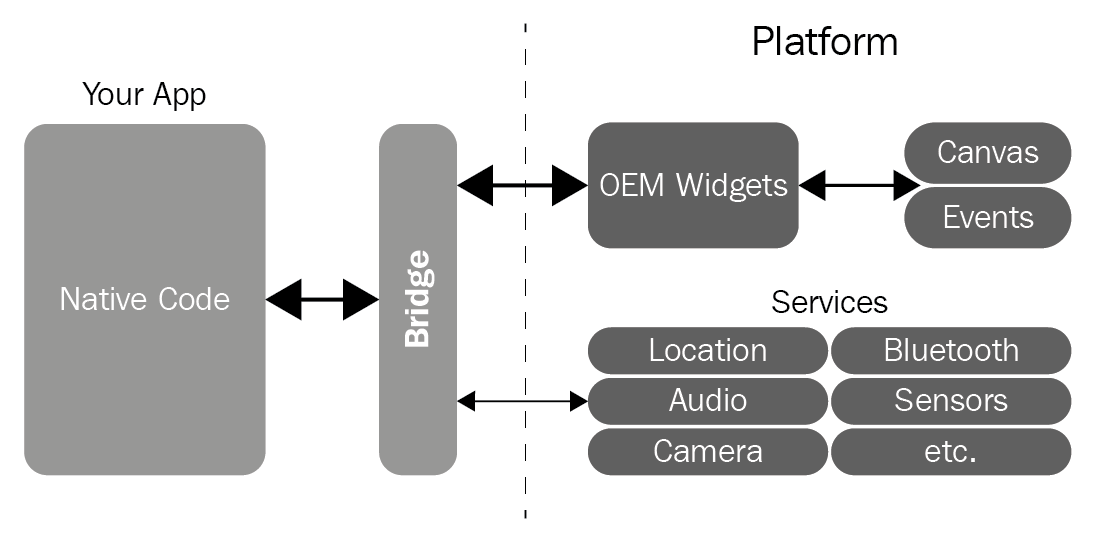
\includegraphics[width=.6\textwidth]{img/interpreted}
    \caption{Interpreted app architecture (Source: \cite{karim_flutter_different})}
    \label{fig:interpreted_architecture}
\end{figure}

\subsubsection*{Cross-compiled approach}

The cross-compiled approach introduces significant changes compared to the previously mentioned solutions. There are no additional layers between the app and the underlying operating system. The Software Development Kit enables the usage of native features and components. A cross-compiled framework uses a programming language of choice which is compiled to native byte code specific to the platform it runs on. Out of the three described approaches, this one should provide the best user experience and performance thus gaining a lot of popularity.  \cite{survey_taxonomy_cross_platform,comparison_technologies_multiplatform,cross_platform_development_study_rn_flutter,eval_rn_flutter}.

\begin{figure}[h]
    \centering
    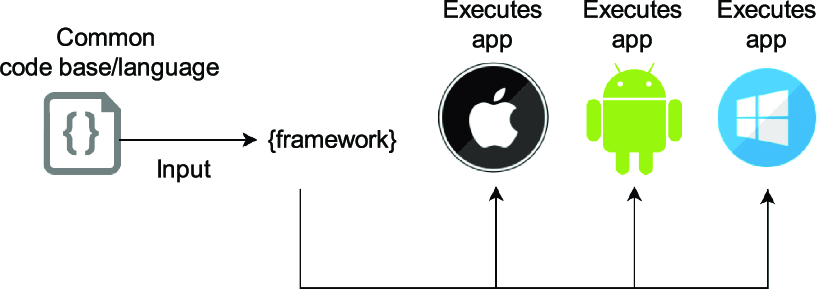
\includegraphics[width=.6\textwidth]{img/cross_compiled}
    \caption{Cross-compiled approach workflow (Source: \cite{survey_taxonomy_cross_platform})}
    \label{fig:cross_compiled_workflow}
\end{figure}

\subsubsection*{Progressive Web Apps}

Progressive Web App (PWA) is a web application that allows the user to install it on a mobile device as if it was a native app. The installation process differs because native apps are downloaded from the app store, while PWAs can be downloaded per request upon the user's visit using a web browser. In order for the web app to acquire the abilities of PWAs, they must fulfill some technical requirements, mainly the implementation of Service Workers and app manifest file. The Service Worker provides some important functions such as the control of data flow (determining whether a web server or locally cached content should be used to complete a request, see Figure \ref{fig:pwa_architecture}). PWA runs in the browser with some features hidden, e.g. address bar, which results in the appearance indistinguishable from native apps. The disadvantage of PWAs is the fact that they cannot provide full support for native components because they are limited by browser APIs. Furthermore, there is a compatibility issue as iOS 11.3 is the minimal compatible version to enable PWA installation.
\cite{survey_taxonomy_cross_platform,comparison_technologies_multiplatform,eval_rn_flutter}.

\begin{figure}[h]
	\centering
	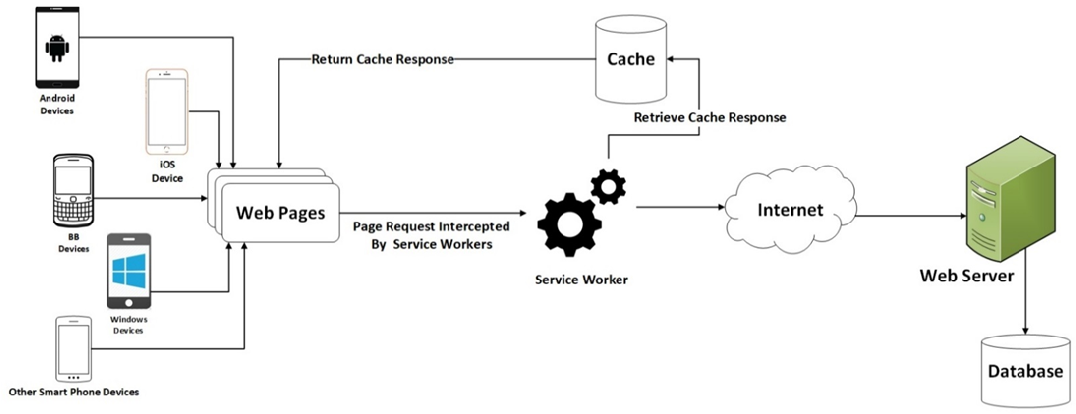
\includegraphics[width=\textwidth]{img/pwa}
	\caption{Progressive Web App architecture (Source: \cite{dawning_pwa})}
	\label{fig:pwa_architecture}
\end{figure}

\subsection{Flutter}



\subsection{React Native}



\subsection{Ionic}



\subsection{Comparison}

% \begin{table}[ht]
% 	\centering
%     \caption{Cross-platform frameworks comparison (Source: Own work based on \dots)}
%     \label{tab:framework_comparison}
% 	\begin{tabular}{ |l|p{30mm}|p{30mm}|p{30mm}| }
% 		\hline
%         \diagbox{Element}{Framework} & Flutter & React Native & Ionic \\
% 		\hline
% 		Initial release&2017&&\\
%         \hline
% 		Current stable version&&&\\
%         \hline
% 		Implemented with&C, C++, Dart&&\\
%         \hline
% 		Supported platforms&Android, iOS, Web, Windows, macOS, Linux&&\\
%         \hline
% 		Supported IDEs??&&&\\
%         \hline
% 		Programming language&Dart&&\\
%         \hline
% 		Rendering&Canvas drawing&Native platform components&Native platform components\\
% 		\hline
% 	\end{tabular}
% \end{table}

\subsection{Evaluation of cross-platform frameworks}

Considering the ongoing changes to the mobile market as well as the saturation of different cross-platform solutions, performing the selection of a specific framework for application development becomes a more and more complicated task. Especially because for each use-case there might be a different optimal solution based on different aspects such as business costs, development limitations, etc. For that reason, a few evaluation methods have been proposed in the literature, some of them very simple and some of them more detailed. There is a lot of scientific work performing the assessment of a selection of available cross-platform frameworks according to those methods. The issue with such evaluation outcome lays in the fact it can become out-dated in a short time with the breaking updates to the considered technologies. For example, a majority of literature on the topic of cross-platform development considers a tool Adobe PhoneGap which has been discontinued and thus is no longer relevant. Therefore, the assessment frameworks themselves are a strong base for performing further research  without the risk of becoming obsolete while the actual assessment ought to be repeated over time to ensure an up-to-date results.

\begin{table}[h]
	\centering
    \caption{Cross-platform frameworks evaluation criteria (Source: Own work based on \cite{rieger_eval_cp})}
    \label{tab:eval_criteria}
	\begin{tabular}{ |l|p{.76\textwidth}| }
		\hline
        \textbf{Perspective}&\textbf{Criteria}\\
		\hline
		Infrastructure&License, Supported target platforms, Supported development platforms, Distribution channels, Monetisation, Internationalisation, Long-term feasibility\\
		\hline
		Development&Development environment, Preparation time, Scalability, Development process fit, User interface design, Testing, Continuous delivery, Configuration management, Maintainability, Extensibility, Integrating custom code, Pace of development\\
		\hline
		App&Access to device-specific hardware, Access to platform-specific functionality, Support for connected devices, Input device heterogeneity, Output device heterogeneity, Application life cycle, System integration, Security, Robustness, Degree of mobility\\
		\hline
		Usage&Look and feel, Performance, Usage patterms, User authentication\\
		\hline
	\end{tabular}
\end{table}

Table \ref{tab:eval_criteria} provides an overview of some of the evaluation criteria proposed in the literature, divided into four perspectives: Infrastructure, Development, App and Usage. The first perspective revolves around licensing, platform support, distribution and long-held operability. Development perspective considers all the aspects directly connected to software development, e.g. available IDEs, learning and implementation effort, scalability, user interface design abilities, maintainability and testing. App perspective includes mainly security, hardware access and external devices. Finally, Usage perspective concerns the aspects connected with end-user experiece such as app appearance and behavior, authentication and performance \cite{eval_rn_flutter,rieger_eval_cp}.

The process of the complete evaluation of a single cross-platform framework according to the above-mentioned criteria is a complex and labor-consuming task perfectly fitting into the methodology of Multi-Criteria Decision Making (MCDM). This methodology can provide a standardized way of approaching the issue of framework selection. Some of the popular solutions for MCDM are Analytic Hierarchy Process (AHP), Technique for Order of Preference by Similarity to Ideal Solution (TOPSIS) or Multi-attribute Utility Theory (MAUT). In the literature there are also proposed approaches created from the merge of a subset of those solutions, e.g. Integrated Multi-Criteria Decision Making \cite{lachgar_mcdm_cp}.
